\documentclass{article}
\usepackage[english]{babel}
\usepackage[utf8]{inputenc}
\usepackage{fancyhdr}
\usepackage{geometry}
\usepackage{enumitem}
\usepackage{amsmath}
\usepackage{graphicx}
\usepackage{tcolorbox}
\usepackage{amssymb}
\usepackage[thinc]{esdiff}
\usepackage{float}

%%%%%%%%%%%%%%%%%%%%%%%%%%%%%%%%%%%%%%%%%%%%%%%%%%%%%%%%%%%%%%%%%%%%%%%%%%%%%%%% DOCUMENT FORMAT

\geometry{letterpaper, portrait, margin=1in}
\graphicspath{ {images/} }
\pagestyle{fancy}
\fancyhf{}
\lhead{Keerthik Muruganandam}
\rhead{Yadavalli Written Work 7}

%%%%%%%%%%%%%%%%%%%%%%%%%%%%%%%%%%%%%%%%%%%%%%%%%%%%%%%%%%%%%%%%%%%%%%%%%%%%%%%% BEGIN DOCUMENT

\begin{document}

\begin{enumerate}[label=\textbf{(7.\arabic*)}]

%%%%%%%%%%%%%%%%%%%%%%%%%%%%%%%%%%%%%%%%%%%%%%%%%%%%%%%%%%%%%%%%%%%%%%%%%%%%%%%% 7.1 PROBLEM STATEMENT

	\item Evaluate the area of the following graph
	\begin{figure}[H]
		\centering
		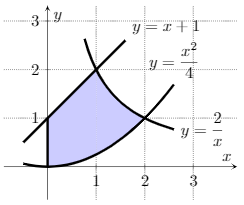
\includegraphics[scale=.75]{triginta}
		\caption{integral area}
	\end{figure}
%%%%%%%%%%%%%%%%%%%%%%%%%%%%%%%%%%%%%%%%%%%%%%%%%%%%%%%%%%%%%%%%%%%%%%%%%%% 7.1 WORK

To solve this, we can use the formula for area between two functions and apply it to the graph above. First, we must split our area into two parts, one from 0 to 1 and another from 1 to 2. Then, our top curves will be $x+1$ and $\dfrac{2}{x}$ for each limit respectively and our bottom curve will be $\dfrac{x^2}{4}$ for both integrals. Setting up what we have described yields
\[\int_0^1\!x+1-\frac{x^2}{4}\,dx+\int_1^2\!\frac{2}{x}-\frac{x^2}{4}\,dx\]
Computing the anti-derivatives of each integral using basic integration rules provides the expression
\[\left[\frac{x^2}{2}+x-\frac{x^3}{12}\right]_0^1+\left[2\ln|x|-\frac{x^2}{12}\right]_1^2\]
Now we can evaluate this to create the value
\begin{align*}
\left(\frac{1^2}{2}+1-\frac{1^3}{12}\right)-\left(\frac{0^2}{2}+0-\frac{0^3}{12}\right)+\left(2\ln|2|-\frac{2^2}{12}\right)-\left(1\ln|1|-\frac{1^1}{12}\right) &= \frac{1}{2}+1-\frac{1}{3}+\ln4 \\
&= \frac{11}{6}+\ln4
\end{align*}
That is the final value for our integral. Thus, the area of Figure 1 is equal to $\dfrac{11}{6}+\ln4$.

%%%%%%%%%%%%%%%%%%%%%%%%%%%%%%%%%%%%%%%%%%%%%%%%%%%%%%%%%%%%%%%%%%%%%%%%%%% NEWPAGE
\newpage
%%%%%%%%%%%%%%%%%%%%%%%%%%%%%%%%%%%%%%%%%%%%%%%%%%%%%%%%%%%%%%%%%%%%%%%%%%% 7.2 PROBLEM STATEMENT

\item Find the arc length of the graph of the function $y=\dfrac{e^x+e^{-x}}{2}$ over the interval $[0,3]$.
%%%%%%%%%%%%%%%%%%%%%%%%%%%%%%%%%%%%%%%%%%%%%%%%%%%%%%%%%%%%%%%%%%%%%%%%%%% 7.2 WORK

First of all, recall the arc length equation, which is to find the length of a function $f(x)$ on $[a,b]$
\[L=\int_a^b\!\sqrt{1+\left(f^\prime(x)\right)^2}\,dx\]
Now let $f(x)=\dfrac{e^x+e^{-x}}{2}$ and $[a,b]=[0,3]$. Computing the derivative of $f(x)$ is accomplished by using derivative rules.
\begin{align*}
\diff{}{x}\left(\frac{e^x+e^{-x}}{2}\right) &= \frac{1}{2}\diff{}{x}\left(e^x+e^{-x}\right)\\
&= \frac{1}{2}(e^x-e^{-x})
\end{align*}
The equation for the arc length is then
\begin{align*}
L &= \int_0^3\!\sqrt{1+\left(\frac{1}{2}(e^x-e^{-x})\right)^2}\,dx \\
&= \int_0^3\!\sqrt{\frac{4+e^{2x}-2+e^{-2x}}{4}}\,dx\\
&= \frac{1}{2}\int_0^3\!\sqrt{e^{2x}+2+e^{-2x}}\,dx\\
&= \frac{1}{2}\int_0^3\!\sqrt{\left(e^x+e^{-x}\right)^2}\\
&= \frac{1}{2}\int_0^3\!e^x+e^{-x}\,dx
\end{align*}
Thus, the integral has simplified into a form which is easily integrable. 
\begin{align*}
\frac{1}{2}\int_0^3\!e^x+e^{-x}\,dx &= \frac{1}{2}\left[e^x-e^{-x}\right]_0^3\\
&= \frac{1}{2}\left(\left(e^3-e^{-3}\right)-\left(e^0-e^{-0}\right)\right)\\
&= \frac{1}{2}\left(e^3+e^{-3}\right)\\
&= \frac{e^3}{2}+\frac{e^{-3}}{2}\\
&= \frac{e^3}{2e^3}
\end{align*}
Therefore,  the arc length of the graph of the function $y=\dfrac{e^x+e^{-x}}{2}$ over the interval $[0,3]$ is $\dfrac{e^3}{2e^3}$

%%%%%%%%%%%%%%%%%%%%%%%%%%%%%%%%%%%%%%%%%%%%%%%%%%%%%%%%%%%%%%%%%%%%%%%%%%% NEWPAGE

\newpage

%%%%%%%%%%%%%%%%%%%%%%%%%%%%%%%%%%%%%%%%%%%%%%%%%%%%%%%%%%%%%%%%%%%%%%%%%%% 7.3 PROBLEM STATEMENT

\item For the function $f(x)=1+\ln x$ on the domain $[a,b]$, where $1\le a<b$,
\begin{enumerate}
\item Find the average value of $f$ on the given domain.
\item Find $c$ such that $f_{ave}=f(c)$.
\end{enumerate}
%%%%%%%%%%%%%%%%%%%%%%%%%%%%%%%%%%%%%%%%%%%%%%%%%%%%%%%%%%%%%%%%%%%%%%%%%%% 7.3 WORK

\begin{enumerate}

\item Once more, remember the formula for average value is 
\[f(c)=\frac{1}{b-a}\int_a^b\!f(x)\,dx\]
Substituting in our specific values yields the integral
\[f(c)=\frac{1}{b-a}\int_a^b\!1+\ln x\,dx\]
Recall that the antiderivative of $\ln x=x\ln x-x$. Then we can do the math
\begin{align*}
f(c) &= \frac{1}{b-a}\int_a^b\!1+\ln x\,dx\\
&= \frac{1}{b-a}\left[x+(x\ln x-x)\right]\\
&= \frac{1}{b-a}\left((b\ln b)-(a\ln a)\right)\\
&= \frac{1}{b-a}\left(\ln{b^b}-\ln{a^a}\right)\\
&= \frac{1}{b-a}\left(\ln{\frac{b^b}{a^a}}\right)\\
&= \frac{\ln\frac{b^b}{a^a}}{b-a}
\end{align*}
Therefore, the average value of $f(x)$ is $\dfrac{\ln\frac{b^b}{a^a}}{b-a}$.
\item Take our equation from before
\begin{align*}
f(c) &= \frac{\ln\frac{b^b}{a^a}}{b-a}
\end{align*}
Let us substitute in $f(x)$ for $f(c)$. Then let us manipulate the equation until it is solving for $c$. Doing this results in
\begin{align*}
1+\ln c &= \frac{\ln\frac{b^b}{a^a}}{b-a}\\
\ln c &= \frac{\ln\frac{b^b}{a^a}}{b-a}-1\\
c &= e^{\frac{\ln\frac{b^b}{a^a}}{b-a}-1}\\
&= \frac{e^{\frac{\ln\frac{b^b}{a^a}}{b-a}}}{e}
\end{align*}
Thus the value of $c=\dfrac{e^{\dfrac{\ln\dfrac{b^b}{a^a}}{b-a}}}{e}$ will make $f(c)=f_{ave}$
\end{enumerate}

%%%%%%%%%%%%%%%%%%%%%%%%%%%%%%%%%%%%%%%%%%%%%%%%%%%%%%%%%%%%%%%%%%%%%%%%%%% NEWPAGE

\newpage

%%%%%%%%%%%%%%%%%%%%%%%%%%%%%%%%%%%%%%%%%%%%%%%%%%%%%%%%%%%%%%%%%%%%%%%%%%% 7.4 PROBLEM STATEMENT

\item \textbf{Professional Problem:} Suppose $f(x)$ is a continuous function. Apply the MVT for derivatives to the function $F(x)=\int_a^x\!f(t)\,dt$ prove the MVT for integrals.
%%%%%%%%%%%%%%%%%%%%%%%%%%%%%%%%%%%%%%%%%%%%%%%%%%%%%%%%%%%%%%%%%%%%%%%%%%% 7.4 WORK

Recall that the MVT for derivatives is
\begin{align*}
f^\prime(c) &= \frac{f(b)-f(a)}{b-a}\mathrm{.}
\end{align*}
Substitution of $F(x)$ into the MVT creates the equations
\begin{align*}
F^\prime(c) &= \frac{F(b)-F(a)}{b-a}\\
&= \frac{\int_a^b\!f(t)\,dt-\int_a^a\!f(t)\,dt}{b-a}\mathrm{.}
\end{align*}
Looking at the equation, recall the FTC Part 1 which states that "If $f$ is continuous on $[a,b]$ and $g(x)=\int_a^x\!f(t)\,dt$ on $[a,b]$, then $g(x)$ is continuous on $[a,b]$, and $g^\prime(x)=f(x)$ on $(a,b)$." Our functions $f(x)$ and $F(x)$ satisfy the conditions for $f(t)$ and $g(x)$ respectively so we can simplify our integral with the FTC. Also remember that and integral with the bounds $[a,b]$ where $a=b$ is 0. 
\begin{align*}
F^\prime(c) &= \frac{\int_a^b\!f(t)\,dt-\int_a^a\!f(t)\,dt}{b-a}\\
f(c) &= \frac{\int_a^b\!f(t)\,dt-\int_a^a\!f(t)\,dt}{b-a}\\
&= \frac{\int_a^b\!f(t)\,dt}{b-a}\\
&= \frac{1}{b-a}\int_a^b\!f(t)\,dt
\end{align*}
The formula for the MVT of integrals is
\[f(c)=\frac{1}{b-a}\int_a^b\!f(t)\,dt\]
Notice that the MVT for integrals and the equation we derived above are exactly the same. Thus, we have proved the Mean Value Theorem for integrals provided the the Mean Value Theorem for derivatives and the Fundamental Theorem of Calculus are true.

%%%%%%%%%%%%%%%%%%%%%%%%%%%%%%%%%%%%%%%%%%%%%%%%%%%%%%%%%%%%%%%%%%%%%%%%%%% END DOCUMENT

\end{enumerate}
\end{document}
